\documentclass[../main.tex]{subfiles}	



\begin{document}
	
\chapter{Extent}
From Wirtinger calculus backpropagation to specific software implementation challenges, in this chapter are described the fundamental details of
complex-valued neural network components and how they are related to existing real-valued network implementations. We will show how existing layers and functionalities can be extended to work also with a complex-valued input and which of them needs to be completely redefined.\\
We address the problem of re-adapting the training process building a complex backpropagation algorithm on top of many prior works, that allows for an optimization when the loss function is real-valued, thanks to Wirtinger calculus.\\
Furthermore, we will discuss in details the problem of building complex-valued activation functions, that was one of the main obstacles in the development of deep learning in this direction.\\
In the end, we will provide a brief presentation of the high level library, built on top of \JAX, that we have realized in order simplify the setup and train of those kind of networks. Nowadays, in fact, the internet is full of deep learning libraries implementing basically every kind of known model, with different optimizations, parallelizations, etc. However, for some reason, many of them still does not provide support to complex data types: a huge obstacle in the growth of complex-valued deep learning.


\section{Problems in the extent}
\label{sec:problems_extent}

Considering just their fundamental structure, complex-valued neural networks work exactly like their real counterpart, and are again constituted by neurons connected among each other (figure \ref{fig:cmplx_neuron}): the only difference is that now those neurons are complex-valued. 

\begin{figure}[!ht]
	\centering
	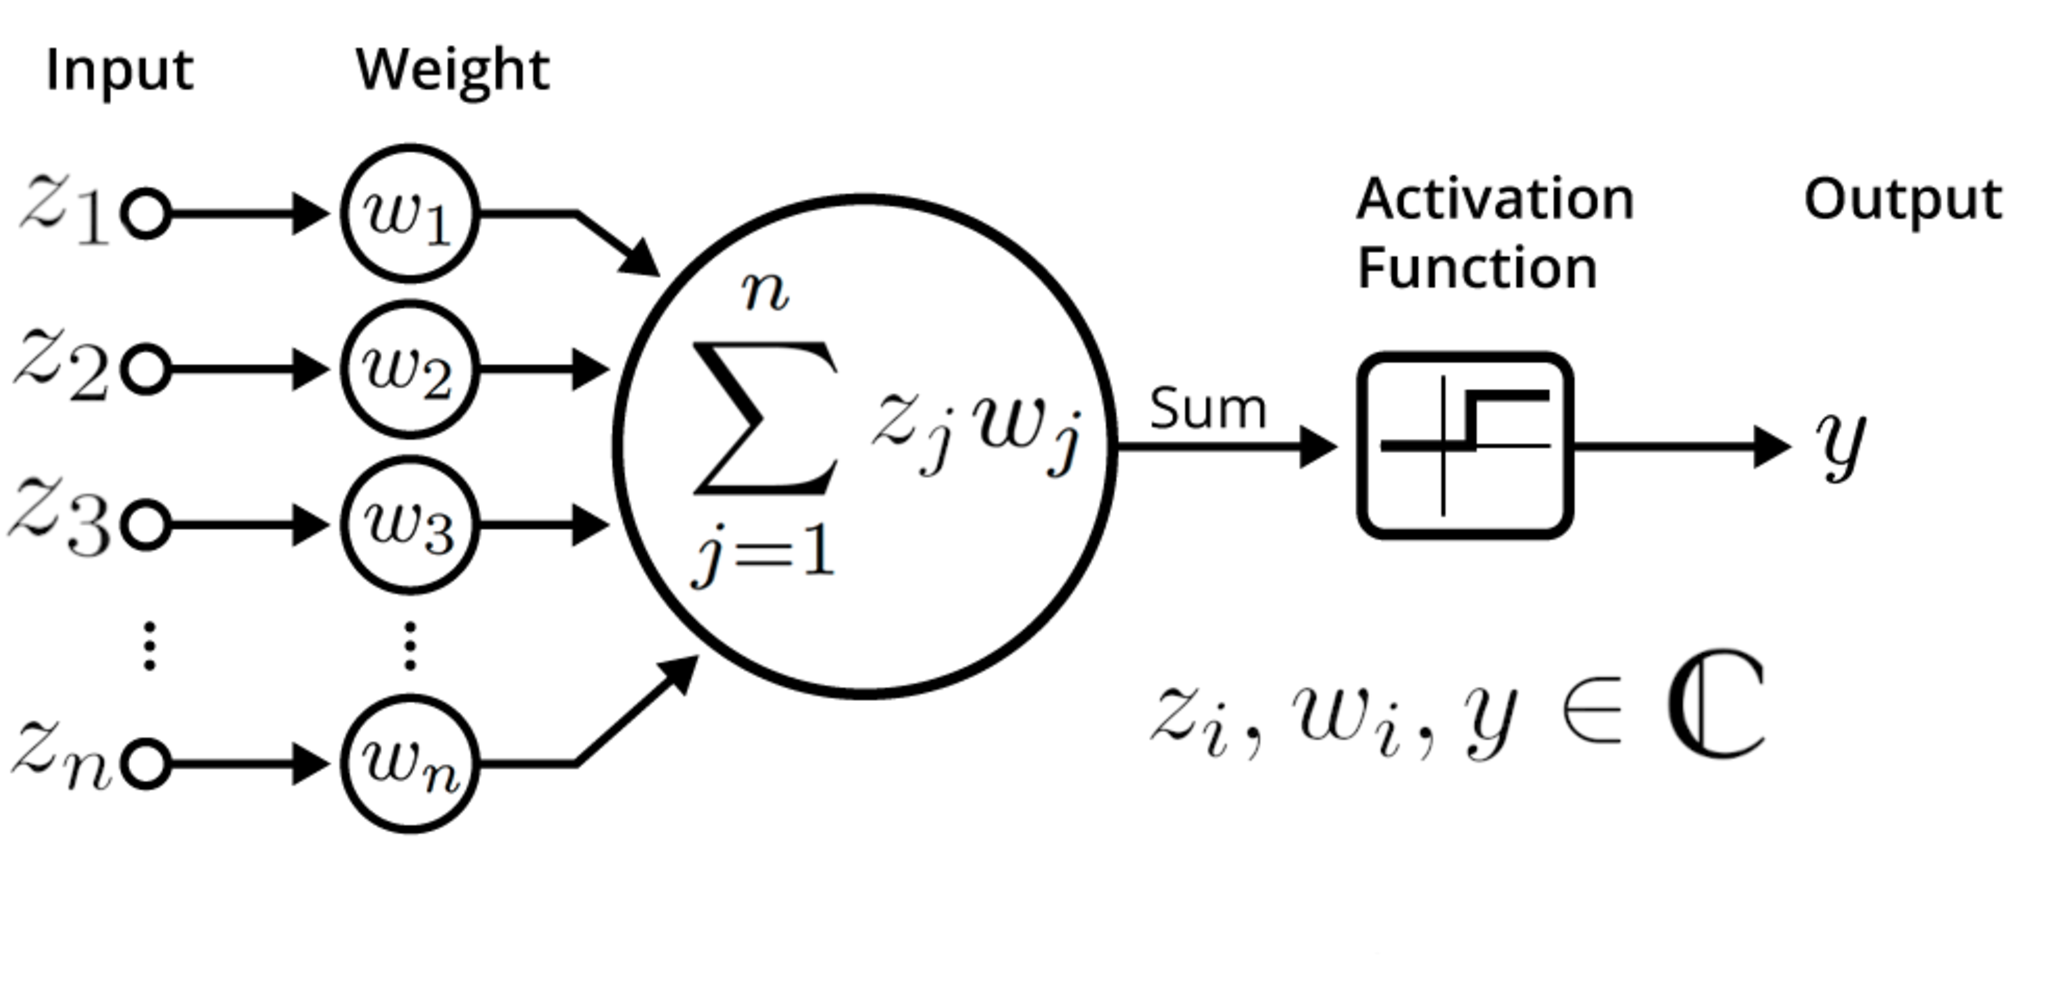
\includegraphics[scale=0.25]{pictures/complex_neuron}
	\caption{Fundamental unit (neuron) of a complex-valued neural network.}
	\label{fig:cmplx_neuron}
\end{figure}

Each neuron receives a weighted input signal $\vb{z}$, that this time is complex valued (as the weights $\vb{w_i}$); this signal in summed up and added to a bias $\vb{b}$, and then passed through an activation function $f:\mathds{C}\to\mathds{C}$, that most of the times is non-linear. If we denote with the subscript $\ell$ the forward pass of a neuron in the $\ell$-th layer, then the output can be expressed with the following formula:
\[ \vb{y}_\ell = f_\ell\left(\sum_{i=1}^{N}\vb{w_i}z_i + \vb{b}_\ell\right) \]
where $N$ are the neurons in layer $\ell$, $M$ the neurons in layer $(\ell-1)$, $\vb{z_{\ell-1}}\in\mathds{C}^M$ was the output of the previous layer, $\vb{w}_\ell\in\mathds{C}^{N\times M}$ and $\vb{b}_\ell\in\mathds{C}^N$ are the learnable parameters of this level, $f_\ell$ the activation function and $\vb{y}_\ell\in\mathds{C}^N$ the effective output.\\
However, when considering a possible extension from $\mathds{R}$ to $\mathds{C}$, we need to take into account a few inconveniences, since we look for a coherent and rigorous framework. 

\subsection*{Max operator is undefined}
As explained also in the introductory mathematical section, $\mathds{C}$ is not an ordered field, in the sense that we cannot define a comparison relation among complex numbers that makes everybody agree. In principle you can define one, like the lexycographical ordering, that compares first the real part and only after the imaginary, or relying on establishing this relation among the magnitudes of those numbers. The latter is actually the preferred approach. This brief overview is important, since many non-linear functions in deep learning, like \texttt{ReLU} and \texttt{Max-Pooling} necessitate of a \textit{maximum} operation in order to fulfill their purpose of increasing numerical stability and dimensionality reduction, respectively.

\subsection*{Unstable Activations}
As we will see in a dedicated section, the problem of defining stable and coherent activation functions is one of the main issues that limited the development of complex-valued deep learning during the years. Complex functions, in fact, necessitate of further limitations to be suitable as activations: because of the Liouville's theorem \ref{th:Liouville}, for example, they can't be limited, and neither grow too slow, otherwise their derivative would always vanish during the backpropagation. So, simply re-adapting existing activations to support complex-valued inputs, maybe redefining ambiguous operations like \texttt{max}, is not enough, especially because you need to care about the eventual loss of complex correlations if the activation is applied independently on the real and imaginary components.

\subsection*{Lost Probabilistic Interpretation}
One nice property of real-valued neural network classifiers is the probabilistic interpretation that we can associate to its final layer, mainly due to the normalization in the range $[0,1]$ provided by sigmoid/softmax activation functions. But now, the final output of the network will be a set of complex numbers, that we cannot interpret anymore as a probability distribution over a set of probabilistic outcomes. This nice property can be partially recovered if we add a \textit{magnitude} layer just before the last activation: in this way we drop all the phase information but we move back to a real-valued problem. Anyway, it always depends on the final objective of the model.

\subsection*{Optimization of a Complex-Valued Output}
Another problem related to having a complex-valued output, beside its interpretation, is the loss associated. If you have a complex final loss, how can you effectively minimize it? In the first chapter we have defined the minimum of a function defined in $\mathds{C}$ as the point $z_0\in\mathds{C}$ in which its modulus is minimized. But this definition, provided by the author of that complex analysis book, is referred to a total ordering in which we refer first to the magnitudes, and so also this is just a convention. Notice that, at the end, minimizing the modulus of a complex loss is equivalent to defining a real-valued loss, i.e. $\mathscr{L}:\mathds{C}\to\mathds{R}$, and minimizing it. And that's exactly what we are going to do when setup a backpropagation.\\

After all this steps, it is clear that we cannot simply reuse deep learning architectures designed for real values without first understanding the complex mathematics in neural networks forward and backward.

\section{Complex Backpropagation}
\label{sec:cmplx_backpropagation}

As anticipated in the introductory section, the interest of researchers in this complex-valued deep learning area started arising many years ago; in fact, the first trial to setup a complex backpropagation algorithm even dates back to 1991 \cite{Nitta_complexBP}. According to the author, not only its algorithm turns out to have an higher convergence speed (and the same generalization performances) with respect to its real counterpart, but also that is able to learn an entire class of transformations (e.g. rotations, similarities, parallel displacements, etc.) that the real method cannot. However, having read the work of Nitta \cite{Nitta_complexBP}, I feel it is better to remark a couple of things, mainly because many years have passed from its publication. First of all, the author used a suboptimal setup:
\begin{itemize}
	\item[-] the network followed one of the "conventional" approaches that we are proving to be unefficient, i.e. treating real and imaginary parts of the data as independent random variables;
	\item[-] he computed the derivatives $\partial f/\partial x$ and $\partial f/\partial y$, instead of relying on Wirtinger calculus \ref{eq:CR_derivs}; even if this is a working alternative to ours, we will see that it is suboptimal;
	\item[-] he relied on "bad" activation functions, since, as told by he himself, many times the algorithm failed to converge.
\end{itemize}
I decided to report his work because it was still one of the first and working attempts to develop a complex backpropagation algorithm, but also because of the purely theoretical analysis realized on the transformations that a complex network can learn. Nitta, managed to teach its networks several transformations in $\mathds{R}^2$, like rotations, reductions and parallel displacements, that the corresponding real-valued model didn't	make. He understood first that this was possible thanks to the higher degrees of freedom offered by complex multiplication (discussed in section \ref{subsec:cmplx_multiplication}). But what I believe it is even more interesting, is the relation that Nitta have found among complex-valued networks and the \textbf{Identity theorem} \ref{th:identity}:\\ 
\textit{``We believe
that Complex-BP networks satisfy the Identity Theorem, that is, Complex-BP networks can approximate complex
functions just by training them only over a part of the
domain of the complex functions."}\\
This means that exploiting holomorphic functions when building a complex-valued network can sometimes impact on its generalization capabilities (since its shape will be rigidly determined by its characteristics on a small local region of its domain) \cite{hirose_cvnn}. Unfortunately, no additional work have been realized on this statement during the years, but I think it is an aspect deserving further attention.\\
In section \ref{sec:cmplx_differentiability} we have discussed about complex differentiability, and we also said that holomorphicity is not a property assured for most functions, and even simple ones, like the square modulus, can be not differentiable in the complex sense. In our architectures we have mainly two sources of \textit{nonholomorphicity}: the loss and the activations. For reasons that will be clearer later on, boundedness and analiticity cannot be achieved simultaneously in the complex domain, and the first feature is often preferred \cite{amin_wirtinger}.\\
An elegant approach that can save computational labor is the usage of Wirtinger calculus to setup optimization problems, solvable via gradient descent, for functions that are not holomorphic but at least differentiable with respect to their real and imaginary components.\\
Also for neural network functions we have a similar problem: requiring them to have complex differentiable properties can be quite limiting, and we should again rely on $\mathds{CR}$-calculus. To complicate matters, the chain rule requires now to compute two terms rather than one (both the $\mathds{R}$-derivative and the conjugate $\mathds{R}$-derivative), causing more than $4x$ calculations during the backward pass.\\
"Fortunately", we can significantly reduce both memory and computation time during complex backpropagation by assuming that our final network loss function is \textit{real-valued}. This is a strong but valid assumption since, as already discussed in section \ref{sec:cmplx_numbers}, minimizing a complex-valued function is an \textbf{ambiguous} operation. Also, minimizing the modulus of a complex loss, as suggested by the magnitude ordering introduced, in the end is exactly like optimizing a real-valued function.\\
But why does it turn out to be more efficient? 

\subsection{Steepest Complex Gradient Descent}
\label{sec:steepest_cmplx_gradient_descent}
In the previous sections we have widely discussed about the fact that complex-valued functions cannot be minimized, and so we ended up with the conclusion that we must use a real-valued loss in order to formulate the training process of a complex model as an optimization problem, in continuation to what happens inside real models.\\
Let's then consider a function $f(z):\mathds{C}\to\mathds{R}$: if we decide to proceed with a gradient descent algorithm, which direction are we supposed to take since there are two different derivatives that one can compute ($\partial/\partial z$ and $\partial/\partial \bar{z}$)?\\
It can be proved (\cite{amin_wirtinger, Hualiang_nonlinear} and appendix \ref{app:cmplx_optim}) that the direction of the \textit{steepest gradient descent} is the \textbf{complex cogradient}, $\vb{\nabla_{\bar{z}}}f$. So, given a function $f$ that depends on a complex random variable $z\in\mathds{C}$, the update rule that minimizes it is:
\begin{equation}
	\vb{z} \leftarrow \vb{z} - \alpha\vb{\nabla_{\bar{z}}}f
	\label{eq:cmplx_gradient_descent}
\end{equation}
where $\alpha\in\mathds{R}$ is the learning rate.

\begin{figure}[!ht]
	\centering
	\includegraphics[scale=0.5]{example-image-a}
	\caption{Complex Gradient Descent.}
	\label{fig:cmplx_gradient_descent}
\end{figure}

In order to provide also a visual representation, in figure \ref{fig:cmplx_gradient_descent} we have considered a simple, non holomorphic, real-valued function like $f(z) = z\bar{z} = \norm{z}^2$, that has a unique global minimum at $z=0+0j$. We have then applied the gradient descent and ascent rules in both directions of the gradient, $\vb{\nabla_z}f$, and the cogradient $\vb{\nabla_{\bar{z}}}f$, in order to verify what said above. In the plot we clearly see that the only direction that approaches the true minimum (starting from a random point in the dominium of $f$) is exactly the one determined by the complex cogradient, while the complex gradient moves in a completely wrong direction. Also considering the ascent rules we observe that the steepest direction maximizing $f$ is again the one determined by the cogradient.

\subsection{Backpropagation with a Real-valued Loss}

With the real-valued loss assumption (proposed in \ref{sec:cmplx_backpropagation}) and the update rule \ref{eq:cmplx_gradient_descent}, complex backpropagation turns out to be quite efficient and not so computationally expensive as we thought in section \ref{sec:cmplx_backpropagation}. The situation can be summarized with table \ref{tab:comparison_backpropagation} and figure \ref{fig:visual_cmplx_backpropagation}.

\begin{table}[!ht]
	\centering
	\begin{tabularx}{\linewidth}{C{0.25\textwidth} C{0.3\textwidth} C{0.45\textwidth}}
		\toprule
		\textbf{Standard Real Calculus} & \textbf{Complex Calculus} & \textbf{Complex Calculus, \arraybackslash assuming real-valued loss}\\
		\midrule
		Input to layer $\ell +1$:
		\[ \pdv{f_L}{x_\ell} \] & \[\pdv{f_L}{z_\ell} \text{  and  } \pdv{f_L}{\bar{z}_\ell}\] & \[ \pdv{f_L}{\bar{z}_\ell}\] \\
		\midrule
		Output from layer $\ell$:
		\[ \pdv{f_L}{x_{\ell-1}} = \pdv{f_L}{x_\ell}\pdv{f_\ell}{x_{\ell-1}}\] & \[ \pdv{f_L}{z_{\ell-1}} = \pdv{f_L}{z_\ell}\pdv{f_\ell}{z_{\ell-1}} + \pdv{f_L}{\bar{z}_\ell}\overbar{\left(\pdv{f_\ell}{\bar{z}_{\ell-1}}\right)}\] \\
		& \[ \pdv{f_L}{\bar{z}_{\ell-1}} = \pdv{f_L}{z_\ell}\pdv{f_\ell}{\bar{z}_{\ell-1}} + \pdv{f_L}{\bar{z}_\ell}\overbar{\left(\pdv{f_\ell}{z_{\ell-1}}\right)}\] & \[ \pdv{f_L}{\bar{z}_{\ell-1}} = \overbar{\left(\pdv{f_L}{\bar{z_\ell}}\right)}\pdv{f_\ell}{\bar{z}_{\ell-1}} + \pdv{f_L}{\bar{z}_\ell}\overbar{\pdv{f_\ell}{z_{\ell-1}}} \] \\
		\bottomrule
	\end{tabularx}
	\caption{Comparison of backpropagation calculus. (source: \cite{Virtue:EECS-2019-126})}
	\label{tab:comparison_backpropagation}
\end{table}

\begin{figure}[!ht]
	\centering
	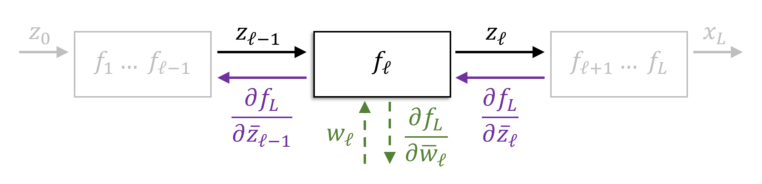
\includegraphics[scale=1.]{pictures/pass_cmplx_layer}
	\caption{Forward and backward pass through a complex layer. (source \cite{Virtue:EECS-2019-126})}
	\label{fig:visual_cmplx_backpropagation}
\end{figure}

Now the algorithm needs to pass only one of the two $\mathds{CR}$ derivatives back to the earlier layers, even tho, because of the chain rule \ref{eq:CR_derivs_chain_rule}, it must compute both of them, at least for the final layer. In figure \ref{fig:visual_cmplx_backpropagation} it is effectively illustrated how input and derivatives flow through the layers during the forward and backward pass, respectively.\\
Given the steepest complex gradient descent rule \ref{eq:cmplx_gradient_descent}, we can then write down the equivalent expression for our network function depending on a set of parameters $\vb{w}$:
\[ \vb{w}_n \leftarrow \vb{w}_n - \alpha\pdv{f}{\bar{\vb{w}}_n} \]

\section{Re-definition of the main neural network layers}

We have started writing down this chapter with the purpose of building a working and coherent framework for complex-valued machine learning. And we also 
In section \ref{sec:problems_extent} we have analyzed the main obstacles that we encounter during this extension, while in \ref{sec:cmplx_backpropagation} we 

\subsection*{Fully-Connected Layers}
For the fundamental layers of a neural network the extension is quite trivial. Consider a layer with $K$ complex-valued units, a weight vector $\vb{w}\in\mathds{C}^K$ and a bias term $\beta\in\mathds{C}$; then, the response to a certain input vector $\vb{z}\in\mathds{C}^N$ (given also the activation function $f$) is:
\[ \vb{y} = f(\vb{z}, \left\{\vb{w},\beta\right\}) = f\left(\sum_k z_kw_k + \beta\right) = f\left(\vb{z}^T\vb{w} + \beta\right) \]

So it is just like the real case, with the only difference that now the multiplication is in $\mathds{C}$ and not in $\mathds{R}$, with all the consequences already discussed in \ref{subsec:cmplx_multiplication}.\\
What we should care about is, instead, the initial values of the networks' parameters. Proper initialization can, in principle, help reducing the risk of vanishing or exploding gradients. Conventionally, researchers follow the approaches proposed by Glorot \cite{xavier_init} or by He \cite{he2015delving} (the latter designed specifically for \texttt{ReLU} activations), with the final objective of ensuring that the variance of input, output and their gradients are the same. According to these two methods, weights should be initialized with a normal distribution (or truncated-normal) with zero mean and standard deviation that depends on the number of units in that specific layer. Thanks to Trabelsi \cite{trabelsi2018deep} (derivation in appendix \ref{app:weight_init}) we could provide two equivalent procedures, but in the complex domain.\\
To put in place them, we need first to consider the weights in polar form, i.e. $\norm{\vb{w}}e^{i\theta}$, and then:
\begin{itemize}
	\item random sampling the magnitude according to a \textbf{Rayleigh distribution} with parameter $\sigma= 1 / \sqrt{n_{in} + n_{out}}$ (\texttt{Complex Xavier} initialization) or $\sigma= 1 / \sqrt{n_{in}}$ (\texttt{Complex He} initialization);
	\item random sampling the phases according to a \textbf{uniform distribution} in $[-\pi,\pi`]$.
\end{itemize}
The biases $\beta$, instead, can all be initialized simply to 0, or uniformly in a small interval $[-\varepsilon, \varepsilon]$.

\subsection*{Convolutional Layers}
In order to perform the equivalent of a traditional real-valued 2D convolution in the complex domain, we convolve a complex filter matrix $\vb{W} = \vb{A}+i\vb{B}$ by a complex vector $\vb{h} = \vb{x}+i\vb{y}$, where $\vb{A}, \vb{B}$ are real matrices and $\vb{x}, \vb{y}$ are real vectors, since we are simulating complex arithmetic using real-valued entries. As the convolution operator is distributive, we have:
\begin{equation}
	\vb{W} * \vb{h} = \left(\vb{A}*\vb{x}-\vb{B}*\vb{y}\right) + i\left(\vb{B}*\vb{x}+\vb{A}*\vb{y}\right)
	\label{eq:cmplx_convolution}
\end{equation}
This is a very nice behavior, since the a complex convolution can be decomposed into two real-valued independent operations. And this means that we can exploit already existing algorithms (like this one, from Gauss \footnote{As explained in this brief \href{https://en.wikipedia.org/wiki/Multiplication\_algorithm\#Complex\_multiplication\_algorithm}{Wikipedia section}, we can reduce the cost of complex multiplication, in some cases.}) to perform efficiently this (already expensive) computation.\\
Notice also that complex convolutional layers' weights basically, can learn to rotate the phase of desirable data toward the positive real axis; in fact, if we rewrite \ref{eq:cmplx_convolution} in a matrix form:
\[ \mqty[\real(\vb{W}*\vb{h}) \\ \imaginary(\vb{W}*\vb{h})] = \mqty[\vb{A} & -\vb{B}\\ \vb{B} & \vb{A}] * \mqty[\vb{x} \\ \vb{y}]	 \]
In figure \ref{fig:cmplx_convolution} we can observe a visual representation of the complex convolution proposed by \cite{trabelsi2018deep}.

\begin{figure}[!ht]
	\centering
	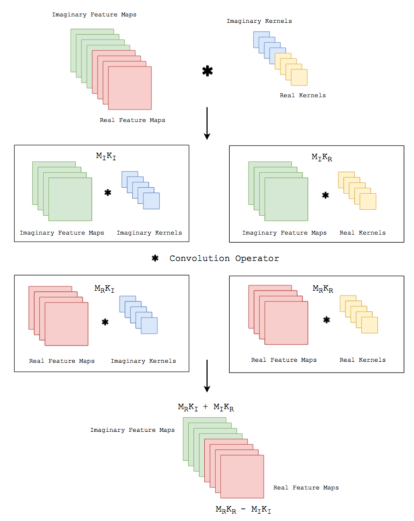
\includegraphics[scale=1.75]{pictures/complex_convolution}
	\caption{Implementation details of the Complex Convolution (by \cite{trabelsi2018deep}).}
	\label{fig:cmplx_convolution}
\end{figure}

In principle, however, even tho complex convolution should have the same computational cost as its real-valued counterpart, in practice it is four times more expensive, just because complex multiplication in the worst case requires four products and two additions.

\subsection*{Pooling Layers}
The pooling operation involves sliding a n-dimensional filter over each channel of the feature map and summarizing the features lying within the region covered by the filter. Pooling layers are essentially dimensionality reduction levels inside the network, with the purpose of making the model more robust to positional variations in the input. \\
There are mainly two kinds of pooling operations that we want to extend to the complex domain:
\begin{itemize}
	\item \texttt{Average Pooling}: replaces the elements in the filtered region of the feature map with their mean. The average of a set of complex number is a well defined operation and so no further work is needed in this case.
	\item \texttt{Max Pooling}: replaces the elements in the filtered region of the feature map with their maximum. In this case, instead, we have that the maximum operation is ambiguous in $\mathds{C}$, and so we must establish an ordering to re-define this layer. Our choice that was to setup the max pooling operation to return the complex number with the highest magnitude, inside the region covered by the filter. Namely:
	\[ \text{MaxPool}(\left\{z_k\right\}) = z_n \qquad\text{where}\; n = \underset{k}{argmax}\;\norm{z_k} \] 
	This choice is not unique, since, as repeated several times, there are more than one total ordering for $\mathds{C}$.
\end{itemize}

\subsection*{Normalization Layers}
Normalization layers are usually inserted inside the architecture of a neural network with the purpose of improving the stability of the network optimization, especially in cases of an high depth, and for a better control of the gradients. In this case the extension not so straightforward, since you need to re-define several statistical objects.\\
In standard \texttt{Batch-Normalization} we train two internal parameters, a scale and an offset, such that each batch of data has zero mean and standard deviation one. This approach, however, is valid only for real data, since it does not guarantee equal variance for both the real and imaginary components, with a resulting distribution turning out to be non-circular. Following the method proposed by \cite{trabelsi2018deep}, the idea is to normalize data to obtain a standard complex normal distribution (basically the one in figure \ref{}), achieved by multiplying the zero-centered data ($\vb{z}-\Ev{\vb{z}}$) by the inverse square root of their $2x2$ covariance matrix $\vb{V}$ \footnote{The existence of the inverse matrix is guaranteed by the positive (semi-) definiteness of $\vb{V}$. Eventually, you can enforce this condition by adding a small quantity $+\varepsilon\mathds{I}$ to the matrix (Tikhonov regularization).}:
\begin{equation}
\tilde{\vb{z}} = \left(\vb{V}\right)^{-\frac{1}{2}}\left(\vb{z}-\Ev{\vb{z}}\right) \qquad\text{where}\quad \vb{V} =  \mqty(\Cov(\Re{\vb{z}}, \Re{\vb{z}}) & \Cov(\Re{\vb{z}}, \Im{\vb{z}}) \\ \Cov(\Im{\vb{z}}, \Re{\vb{z}}) & \Cov(\Im{\vb{z}}, \Im{\vb{z}}))
\label{eq:cmplx_batchnorm}
\end{equation}
From a practical point of view, the implementation is the same of the real case. You have again two trainable parameters: $\beta\in\mathds{C}$, i.e. the complex mean, and $\gamma\in\mathds{C}^2$, the complex-valued positive-defined covariance matrix. The \texttt{complex batchnorm} operation is then defined as
\[ BN(\vb{z}) = \gamma\vb{z} + \beta \]
We need, however, to be careful when relying on batchnormalization. This procedure allows, in fact, to avoid co-adaptation between real and imaginary parts of data, effectively reducing the risk of overfitting. But there is a cost to this, since you are basically decorrelating your complex data, partially losing the advantage over two-channels networks \cite{cogswell2016reducing}.\\
For this reason, we sometimes prefer to rely on other kind of normalization layers that, instead, allows to preserve complex data correlations.\\
In simple \texttt{Complex Normalization} we scales a complex scalar input $\vb{z}$ such that its magnitude is set to one, while the phase remains unchanged. In practice we project $\vb{z}$ onto the unit circle. The forward pass is then
\[ \hat{\vb{z}} = e^{i\angle \vb{z}} = \frac{\vb{z}}{\norm{\vb{z}}} = \frac{\vb{z}}{(\vb{z}\bar{\vb{z}})^{1/2}} \]

\subsection*{Other Layers}
There are many layers that do not need any further re-definition to work also in the complex domain: \texttt{Dropout}, Pad or Attention layer, for example. There are also many other structures that should be re-derived (e.g Recurrent layers, LSTM, etc.), but that were out of our scope and so we haven't examined. This should be interpreted just as a starting point in the development of an higher level complex-valued deep learning framework.

\section{Complex-Valued Activation Functions}
One of the main issues encountered in the last 30 years in the developing of a complex-valued deep learning framework was exactly the definition of reliable activation functions. The extension from the real-valued domain turned out to be quite challenging: because of the Liouville's theorem \ref{th:Liouville}, in fact, stating that the only complex-valued functions that are bounded and analytic everywhere are constants, one have necessarily to choose between boundedness and analyticity, in the design of those activations. Furthermore, before the introduction of ReLU, almost all the activation functions known in the real case were bounded. And for the same ReLU the extent was not trivial, since operations like \textit{max} are not defined in the complex domain, Additionally, with complex-valued outputs, we have lost the probabilistic interpretations that functions like \texttt{sigmoid} and \texttt{softmax} used to provide.\\
We have to say, however, that most of the candidate functions that have been proposed, have been developed in a split fashion, i.e. by considering the real and imaginary parts of the activation separately. But, as discussed also in the previous chapter, this approach should be abandoned, since you risk losing the complex correlations stored in those variables.\\
In this section, we will explore a few complex-valued activations proposed during the years: first with the ones that are direct extensions of their real counterparts, and then with more "abstract" candidates, that have more reasons to live and work in the complex domain.

\subsection*{Extent from the real case}
The first class of viable approaches consists into barely extending real-valued activations in the complex domain, like the \texttt{sigmoid} and the \texttt{hyperbolic tangent}:
\[ \sigma_\mathds{C}(z) = \frac{1}{1+e^{-z}}  \qquad\qquad \tanh(z) = \frac{e^z - e^{-z}}{e^z + e^{-z}} \]
These functions are fully-complex, and also analytic and bounded almost everywhere, at the cost of introducing a set of singular points: both function, in fact, seems to diverge periodically in the imaginary axis of the complex plane. Limiting and scaling carefully the input values seems to help avoiding then those singularities and so partially containing the instability. However, I believe that there are simpler and more efficient alternatives.

\subsection*{Separable Activations}
As already explained, the main tendency in the development of complex-valued activation functions was basically getting back the "old" designs for real-valued models and using them independently on the real and imaginary components of the input.\\
This can be done easily with both the sigmoid and the hyperbolic tangent, mapping real and imaginary parts among input and output as they were independent channels:
\[ f(\vb{z}) = g\left(\Re(\vb{z})\right) + ig\left(\Im(\vb{z})\right), \qquad\text{where}\quad g(x) = \frac{1}{1+e^{-x}} \quad\text{or}\quad g(x)=\tanh(x) \]
Notice that this approach maps the phase of the signal into $[0,2\pi]$, since the function $g$ returns always a positive value.\\
There are also interesting variations to the separable sigmoid, properly designed to work using a complex-valued network on real-valued data. But, for this reason, they are functions with values in $\mathds{R}$ and not in $\mathds{C}$, and so we won't go through them in this work.\\
After the advent of the ReLU activation functions, two designs where developed in this fashion, the \texttt{$\mathds{C}$ReLU} and the \texttt{$z$ReLU}:
\[ \mathds{C}ReLU(z) = ReLU(\Re(z)) + iReLU(\Im(z)) \qquad\qquad zReLU = \begin{cases} z\quad \text{if } \theta_z\in[0,\pi/2] \\ 0\quad\text{otherwise} \end{cases} \]
These functions also share the nice property of being holomorphic in some regions of the complex plane: \texttt{$\mathds{C}$ReLU} in the first and third quadrants, while \texttt{$z$ReLU} everywhere but the set of points $\left\{\Re(z)>0,\, \Im(z)=0\right\} \cup \left\{\Re(z)=0,\, \Im(z)>0\right\}$.

\subsection*{Phase-preserving Activations}
Phase-preserving complex-valued activations are those functions that usually act only on the magnitude of input data, preserving the pre-activated phase during the forward pass. Those are usually non-holomorphic, but at least bounded in the magnitude. They are all based on the intuition that, altering the phase could severely impact the complex representation.\\
The first proposal is the so called \texttt{siglog} activation function:
It is called in this way because it is equivalent to applying the sigmoid to the log of the input magnitude and restoring the phase:
\[ siglog(z) = g\left(\log\norm{z}\right)e^{-i\angle z}= \frac{z}{1+\norm{z}}, \qquad\text{where}\quad g(x) = \frac{1}{1+e^{-x}} \]
Unlike the sigmoid and its separable version, the siglog projects the magnitude of the input from the interval $[0, \infty)$ to $[0,1)$. The authors of this proposal suggested also the addition of a couple of parameters to adjust the \textit{scale}, $r$, and the \textit{steepness}, $c$, of the function:
\[ siglog(z; r,c) = \frac{z}{c + \frac{1}{r}\norm{z}} \]
The main problem with \textit{siglog} is that the function has a nonzero gradient in the neighborhood of the origin of the complex plane, which can lead to gradient descent optimization algorithms
to continuously stepping past the origin rather then approaching the point and staying here.\\
For this reason, an alternative version have been proposed, this time with a better gradient behavior (approaching zero as the input approaches zero), that goes under the name of \texttt{iGaussian}.
\[ iGauss(z;\sigma^2)=g(z;\sigma^2)n(z) \qquad\text{where}\quad g(z;\sigma^2)=1-e^{-\frac{z\bar{z}}{2\sigma^2}},\quad n(z) = \frac{z}{\norm{z}} \]
This activation is basically an inverted gaussian (and this is the reason for which it is more smooth around the origin) and so depends only on one parameter, i.e. its standard deviation $\sigma$.\\
The last activation that we want to consider for this class is another variation of the rectified linear unit, this time called \texttt{modReLU}:
\[ modReLU(z) = ReLU(\norm{z} + b)e^{i\theta_z} = \begin{cases} \left(\norm{z}+b\right)\frac{z}{\norm{z}}\quad\text{if }\norm{z}+b\ge 0 \\ 0\qquad\qquad\qquad\text{otherwise} \end{cases} \]
where $z\in\mathds{C}$, $\theta_z$ is the phase of $z$, and $b\in\mathds{R}$ is a learnable parameter. The idea of this activation is to create a "dead zone" of radius $b$ around the origin, where the neuron will be inactive, while it will be active outside. We decided to consider this function, even if apparently was designed for Recurrent neural networks.

\subsection*{Complex Cardioid}
Even if the \texttt{iGaussian} has nice gradients properties around the origin in the complex plane, the same cannot be said when in input are given large values: in that situation there is high risk of vanishing gradients, the same that have historically hindered the performances of sigmoid-like activations.\\
Because of this, recently a new complex activation function have been proposed: the \texttt{Complex Cardioid} \cite{Virtue:EECS-2019-126}. The cardioid acts as an extension of the ReLU function to the complex domain, rescaling from one to zero all the values with non-zero imaginary component, based on how much the same input is rotated in phase with respect to the real axis. Also, the cardioid is sensitive to the input phase, rather than the modulus: the output magnitude is, in fact, attenuated based on the input phase, while the output phase remains equal to the original one.\\
The analytical expression for this activation function is:
\[ cardioid(z) = \frac{1}{2}\left(1 + \cos(\angle z)\right)z \]
Another very nice property is that when the inputs are restricted to real values, this function becomes simply the ReLU activation.\\
We will see, in our applications, that the cardioid effectively allows complex networks to converge in a fast and also stable way.

\subsection*{A brief recap}

\begin{table}[!ht]
\centering
\begin{tabular}{c c c}
\toprule
\textbf{Activation} & \textbf{Analytic Form} & \textbf{Reference}\\
\midrule
Sigmoid & $\sigma(z)$ & // \\
Hyperbolic Tangent & $\tanh(z)$ & // \\
Split-Sigmoid & $\sigma(\Re(z)) + i\sigma(\Im(z))$ & \cite{Nitta_complexBP}\\
Split-Tanh & $\tanh(\Re(z)) + i\tanh(\Im(z))$ & \cite{Nitta_complexBP}\\
$\mathds{C}$ReLU & $ReLU(\Re(z)) + iReLU(\Im(z))$ & \cite{trabelsi2018deep} \\
$z$ReLU & $z\;\text{if } z\in[0,\pi/2],\quad0\quad\text{otherwise}$ & \cite{guberman2016complex} \\
Siglog & $\sigma(\log\norm{z})e^{-i\theta_z}$ & \cite{Koutsougeras_siglog} \\
iGauss & $\left(1-e^{-\frac{z\bar{z}}{2\sigma^2}}\right)\frac{z}{\norm{z}}$ & \cite{Virtue:EECS-2019-126}\\
modReLU & $ReLU(\norm{z} + b)e^{i\theta_z}$ & \cite{DBLP:journals/corr/ArjovskySB15} \\
Cardioid & $\frac{1}{2}\left(1 + \cos(\angle z)\right)z$ & \cite{Virtue:EECS-2019-126}\\
\bottomrule
\end{tabular}
\caption{Recal of the most popular complex-valued activation functions.}
\label{tab:cmplx_activations}
\end{table}

\section{JAX Implementation}

From a practical perspective, in order to setup and realized all the studies and analysis we are going to present, I had to realize a dedicated \texttt{Python} library.\\
In the previous sections we have analyzed all the theoretical obstacles that researchers had to overcome in order to develop a working complex-valued deep learning framework. But, in reality, there are many drawbacks also at the implementation level: first of all the most popular hardware acceleration architectures, \texttt{CUDA} and \texttt{CuDNN} doesn't own a native support for complex-valued data types. And this is by itself a huge limitation, since we cannot train our networks efficiently, and we will have to rely on simple models with few parameters.\\
Regarding existing deep learning libraries, like \texttt{Keras}, \texttt{TensorFlow} and \texttt{Pytorch}, we have to say that they provide a lot of interesting high-level architectures to setup deep learning algorithms, and also they "officially" support complex inputs. Even better, they support complex derivatives. But when you try to implement an effective complex-valued network, you understand how much are they far from an effective comprehensive support (just some known issues: \href{https://github.com/pytorch/pytorch/issues/33152}{1}, \href{https://github.com/tensorflow/tensorflow/issues/17097}{2}, \href{https://github.com/microsoft/tensorflow-directml/issues/32}{3}): regardless of the many errors you can get from structures that should work, from an accurate analysis of the source code of the main layers, you notice that many operations are ambiguous or at least not compatible with the reasoning we adopted to develop the layers extents in this chapter. We could have probably found a way to redefine or override those structures, but we felt that modifying a so large and complex library, without getting undesired side effects, would have been too much work.
\begin{wrapfigure}{r}{0.5\textwidth}
	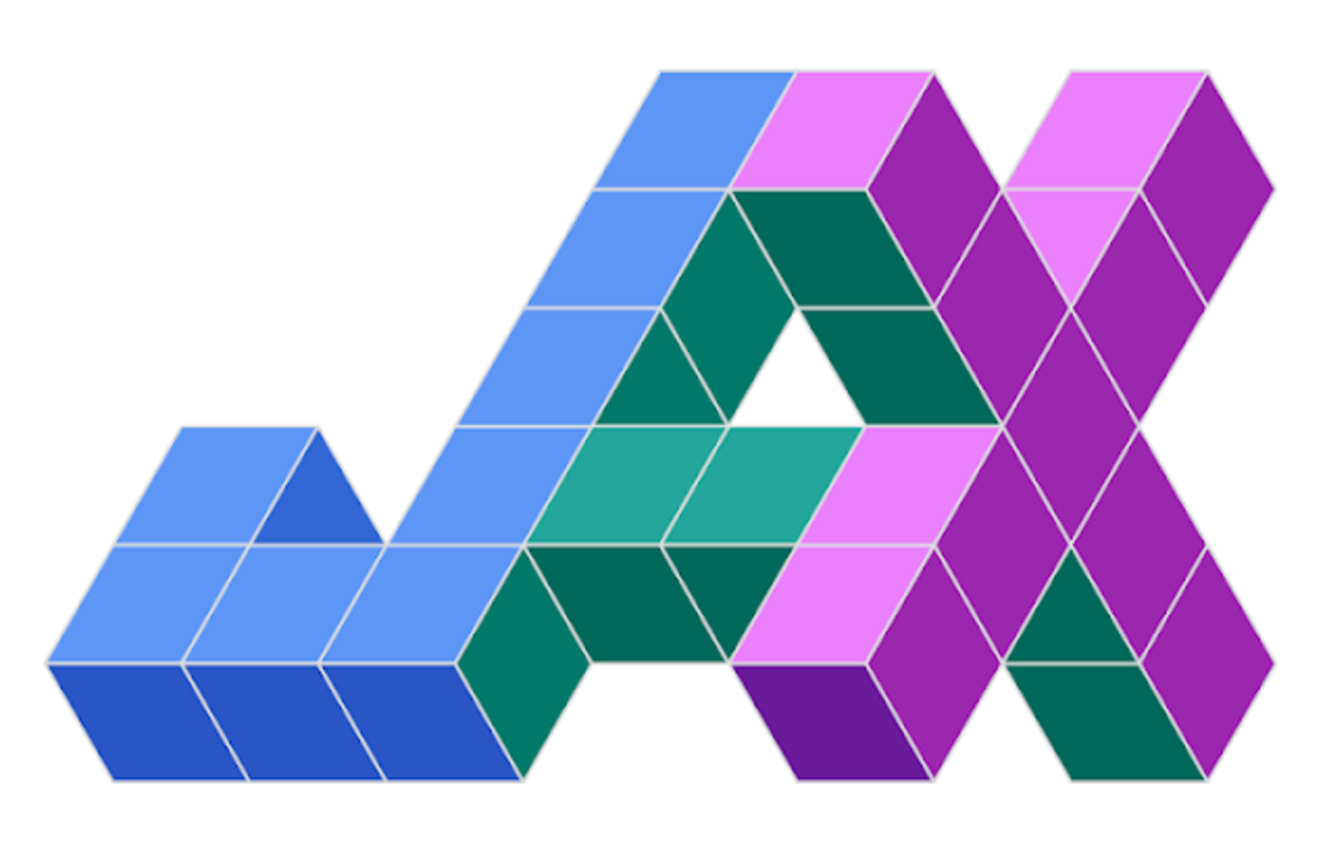
\includegraphics[width=0.5\textwidth]{pictures/JAX_logo.pdf}
	\caption{JAX logo.}
\end{wrapfigure}
For this reason we had to rely on a more niche library, called \texttt{JAX}, and recently developed by \texttt{Google DeepMind}. JAX is \href{https://github.com/hips/autograd}{\textbf{Autograd}} and \href{https://www.tensorflow.org/xla}{\textbf{XLA}} (a domain-specific compiler for linear algebra designed for TensorFlow models), brought together for high-performance numerical computing and machine learning research. It provides composable transformations of Python and NumPy programs: differentiate, vectorize, parallelize, Just-In-Time compile to GPU/TPU, and more. The main advantages that we found using JAX were:
\begin{itemize}
	\item[-] it supports and optimize complex differentiation, for holomorphic and non functions;
	\item[-] it is extremely optimized, with XLA + JIT that partially compensate the lack of native hardware acceleration;
	\item[-] many complex operations/layers are already supported and well defined.
\end{itemize}
More specifically, for building our complex-valued neural networks we will rely on \texttt{dm-haiku}, another library built on top of JAX with the purpose of covering the same role that \href{https://github.com/deepmind/sonnet}{\texttt{Sonnet}} (widely used ad DeepMind) has for Tensorflow, and to simplify the approach of users that are familiar with object oriented programming.\\
Since these are quite recent libraries, and also a definitive approach to complex-valued deep learning does not exists yet, I made a careful and complete analysis of the source code of Haiku and of the most important JAX functions. Thanks to this I effectively noticed that much work is still needed: even if in a small quantity respect to Tensorflow/Pytorch, also in this case many operations turns out to be ambiguous or bad-defined for complex-valued data types (e.g. the \texttt{square} or the \texttt{max} operators). Many of them are also completely undefined (e.g. initialization or, more in general, random complex distributions). We still decided to proceed with JAX mainly because of its flexibility, and many new functions/operations can be redefined without caring of implicit undesired side effects. This is possible also thanks to the design of the training loop, that is quite "explicit" and customizable.\\
From a practical point of view, I had basically to realize small a `\texttt{complex\_nn}' library on top of Haiku, containing the definitions (and re-definitions) of all the necessary components of a complex-valued neural network:
\begin{itemize}
	\item \texttt{layers}: the adaptations derived before for linear, convolutional, pooling and normalization operations;
	\item \texttt{activations}: all functions listed in table \ref{tab:cmplx_activations};
	\item \texttt{initializers}: weights initializers following uniform or truncated random normal distributions, together with the modified approaches described above by Xavier and He;
	\item \texttt{metrics}: categorical accuracy and categorical cross-entropy, useful for the successive classifiers designs; 
	\item \texttt{optimizers}: a \textit{complex-Adam} algorithm;
	\item a \texttt{classifier wrapper} with the purpose of collecting all the necessary functions to setup a training loop with JAX and Haiku;
	\item for completeness, also some utility functions, mainly to realize plots or wrapping more complex structures. 
\end{itemize}
This code has been tested over several datasets. There are in fact a few \texttt{Jupyter Notebooks} providing a detailed explanation of analysis we are going to see, together with some basic setup of some learning procedures.\\
All the implementation and complete analysis is actually available at my gitlab page \footnote{\href{https://gitlab.fbk.eu/mpujatti/complex-valued-deep-learning-for-condition-monitoring}{https://gitlab.fbk.eu/mpujatti/complex-valued-deep-learning-for-condition-monitoring}}.


\end{document}
 